\section{Технологическая часть}

В данном разделе будет описан выбор технологий для разработки и развёртывания базы данных и приложения, а также будут приведены детали реализации ПО.

\subsection{Выбор СУБД}

% PostgreSQL --- основное хранилище, Redis --- кеш данных текущей сессии (по окончании сессии перекидывается на диск на стороне сервера (после возврата из функции обработки подключения, т.е. на стороне сервера надо разделять (идентифицировать) конкретные сессии (не пользователей!))).

\subsubsection{Долговременное хранение данных}

В качестве основного хранилища данных была выбрана объектно-реля-\\ционная СУБД PostgreSQL \cite{PostgreSQL}, которая позволит реализовать многослойную структуру хранения данных. Также стоит отметить, что PostgreSQL сертифицирована ФСТЭК России \cite{fstec} и имеет открытый исходный код.
% поддерживает функции поддержки безопасности и другие многочисленные расширения

% А чего эта сертификация даёт?
% Как и любая сертификация - возможность использования на тех предприятиях, где наличие такого сертификата для ПО необходимо.

\subsubsection{Кеширование данных}

Для хранения данных пользовательских сессий было выбрано in-memory хранилище Redis \cite{Redis}. Данная СУБД удовлетворяет необходимым требованиям (хранилище типа ключ-значение в оперативной памяти) и не требует дополнительной настройки для начала использования.

\subsubsection{Хранение логов системы}

В качестве СУБД для хранения логов была выбрана СУБД-ВР InfluxDB \cite{InfluxDB}. В отличие от PostgreSQL, InfluxDB более компактно хранит данные и оптимизирована на запись данных, что подходит для организации сервера логов.

%Нативная СУБД-ВР представляет собой самостоятельную проприетарную или свободную разработку с оригинальными языком запросов, машиной баз данных, системой хранения данных и др. Представителями данного класса являются системы InfluxDB [19, 27], Kdb+ [29], Prometheus [5, 47], Druid [68], LittleTable [51], FluteDB [34], PhilDB [37], EdgeDB [69], TSMMDB [33] и др.

В InfluxDB данные представляются в виде двумерной таблицы \cite{time_series}, называемой измерением (measurement). В измерении имеется столбец с метками времени (timestamp). Остальные столбцы измерения могут принадлежать одной из двух категорий: поле или тег. Поле (field) хранит данные временного ряда и состоит из ключей (field keys) и значений (field values). Тег (tag) представляет собой метаданные поля и состоит из ключей тегов (tag key) и значений тегов (tag values). Поля не индексируются, но для тегов могут быть созданы индексы. В InfluxDB отсутствует явная схема базы данных.

В InfluxDB поддерживаются понятия серии и точки \cite{time_series}. Серия (series) представляет собой набор данных, имеющих общие измерение, набор тегов и ключи полей. Точка (point) представляет собой элемент данных, состоящий из следующих компонентов: измерение, набор тегов, набор полей, метка времени. Точка однозначно идентифицируется по ее серии и метке времени. При добавлении точек данных метки времени добавляются автоматически.

Хранение данных на физическом уровне в InfluxDB основано на использовании древовидной структуры данных LSM (Log-structured merge-tree) \cite{log_tree}, которая используется в реляционных СУБД и обеспечивает быстрый доступ к данным в случае сценария работы, предполагающего частые запросы на вставку данных. В InfluxDB также поддерживается автоматическое сжатие данных для минимимизации объема хранимых данных. \cite{time_series}

В InfluxDB используется SQL-подобный язык запросов InfluxQL \cite{InfluxQL}, который поддерживает непрерывные запросы (continous query) --- запросы, которые запускаются автоматически с заданной периодичностью.



\subsection{Средства реализации}

Система, взаимодействующая с базой данных, представляет собой веб-сервер, доступ к которому осуществляется с помощью REST API. Для реализации был выбран язык программирования Golang \cite{Golang}, созданный для разработки микросервисных веб-приложений. Далее будет описана разработка микросервиса, предназначенного для хранения данных. 

Для взаимодействия с базами данных будут использоваться драйвера, написанные для языка Golang, предоставляющие интерфейс взаимодействия посредством языка программирования.

Для реализации REST API будет использоваться веб фреймворк gin \cite{Gin}. Документирование REST API будет осуществляться с помощью Swagger \cite{Swagger}, который поддерживает протокол openAPI \cite{openAPI}.

Для развёртывания приложения был выбран оркестратор Docker контейнеров Docker Compose \cite{Docker_compose}. Docker контейнер позволяет изолировать приложение и разворачивать его на любой машине, независимо от окружения. Это реализуется благодаря инкапсуляции всех требуемых зависимостей внутри контейнера. Docker Compose связывает контейнеры в единую систему и позволяет запускать приложение, состоящее из Docker контейнеров. В отдельных контейнерах будут развёртываться следующие службы.

\begin{enumerate}[label*=\arabic*.]
	\item Микросервис приложения, осуществляющего доступ к данным.
	\item PostgreSQL для долговременного хранения данных.
	\item Redis для кеширования данных пользовательских сессий.
	\item InfluxDB для хранения логов системы.
	\item Swagger для документирования REST API.
	\item PgAdmin для администрирования PostgreSQL.
\end{enumerate}

% Внешние средства для мониторинга состояния системы: Docker Desktop (или UI сервиса, на котором развёрнуто приложение), Grafana, PGAdmin.



\subsection{Детали реализации}

\subsubsection{Роли базы данных}

% Реализация ролевой модели (инициализация ролей и выдача им прав).

В конструкторской части была разработана ролевая модель, в которой выделены роли студента, преподавателя и администратора. Сценарий создания ролей и выделения им прав, соответствующих описанной ролевой модели, представлен в приложении В.

% **Скрипт инициализации ролевой модели базы данных для таблиц на каждом слое**

\subsubsection{Хранимая процедура базы данных}

% Реализация хранимой процедуры (инициализация + вызов).

В конструкторской части была разработана хранимая процедура, осуществляющая добавление нового слоя разметки текстов. PL/pgSQL \cite{plpgsql} --- процедурного расширения языка SQL, используемого в СУБД PostgreSQL. Код функции представлен в приложении Г.

\subsubsection{Интерфейс приложения}

% Описать API бекенда.

Разрабатываемая система является серверным приложением, которое принимает запросы клиентов, обрабатывает их и возвращает ответ. Клиенты могут взаимодействовать с сервером через интерфейс REST API, который обеспечивает доступ к разрабатываемой базе данных. 

% (отсылка к 1.2?)

Описание REST API, соответствующего требованиям к проектируемому приложению, представлено в таблице \ref{tbl:rest-api}.

\begin{landscape}
	\begin{longtable}{|p{0.29\textwidth}|p{0.18\textwidth}|p{0.955\textwidth}|}
		\caption[Описание REST API реализуемого приложения]{Описание REST API реализуемого приложения}
		\label{tbl:rest-api}\\
		\hline
		Путь & HTTP-метод & Описание \\
		\endfirsthead
		
		\multicolumn{3}{l}
		{{\tablename\ \thetable{} -- продолжение}} \\\hline 
		Путь & Метод & Описание \\
		\endhead
		
		\multicolumn{3}{|r|}{{Продолжение на следующей странице}} \\ \hline
		\endfoot
		
		\hline \multicolumn{3}{|r|}{{Конец таблицы}} \\ \hline
		\endlastfoot
		\hline
		/api/v1/login         		& POST 		& Вход в систему \\\hline
		/api/v1/logout            	& POST 		& Выход из системы \\\hline
		
		/api/v1/layers/all    		& GET 		& Получение всех слоёв разметки текстов \\\hline
		/api/v1/layers              & POST		& Добавление слоя разметки текстов\\\hline
		
		/api/v1/elements/all    	& GET 		& Получение всех элементов структурных моделей заданного слоя разметки текстов \\\hline
		/api/v1/elements           	& POST		& Добавление элементов структурных моделей заданного слоя разметки текстов\\\hline
		
		/api/v1/models/all    		& GET 		& Получение всех структурных моделей заданного слоя разметки текстов \\\hline
		/api/v1/models              & POST		& Добавление структурных моделей заданного слоя разметки текстов\\\hline
		
		/api/v1/properties/all    	& PUT 		& Получение всех характеристик единиц языка \\\hline
		/api/v1/properties/unit    	& PUT 		& Получение характеристик заданной единицы языка \\\hline
		/api/v1/properties         	& POST		& Добавление характеристик единиц языка\\\hline
		
		/api/v1/units/all    		& PUT 		& Получение всех единиц языка на заданном слое разметки текстов \\\hline
		/api/v1/units/models    	& PUT 		& Получение единиц языка на заданном слое разметки текстов, соответствующих заданным структурным моделям \\\hline
		/api/v1/units/properties    & PUT 		& Получение единиц языка на заданном слое разметки текстов, соответствующих заданным характеристикам \\\hline
		/api/v1/units              	& POST, PATCH& Добавление и редактирование единиц языка на заданном слое разметки текстов\\\hline
		
		/api/v1/users            	& POST 		& Регистрация пользователя в системе \\\hline
		
		/api/v1/admin/stat        	& GET 		& Получение информации о состоянии веб-сервера \\
	\end{longtable}
\end{landscape}

\subsection{Сборка и развёртывание приложения}

% Инструкция по деплою + текст файла docker-compose.

Для сборки частей системы использовались Docker контейнеры, конфигурации которых представлены в приложении Д. Для их развертывания использовался Docker Compose. Листинг конфигурации в формате YAML представлен приложении Е.

\subsection{Примеры работы ПО}

Для разработанного REST API была написана документация с помощью фреймворка \cite{Swagger}, который позволяет не только интерактивно просматривать спецификацию, но и отправлять запросы к приложению с помощью Swagger UI \cite{Swagger_UI}. На рисунках \ref{fig:swagger_main}-\ref{fig:swagger_form_response} представлены примеры работы с Swagger UI.

\begin{figure}[h]
	\centering
	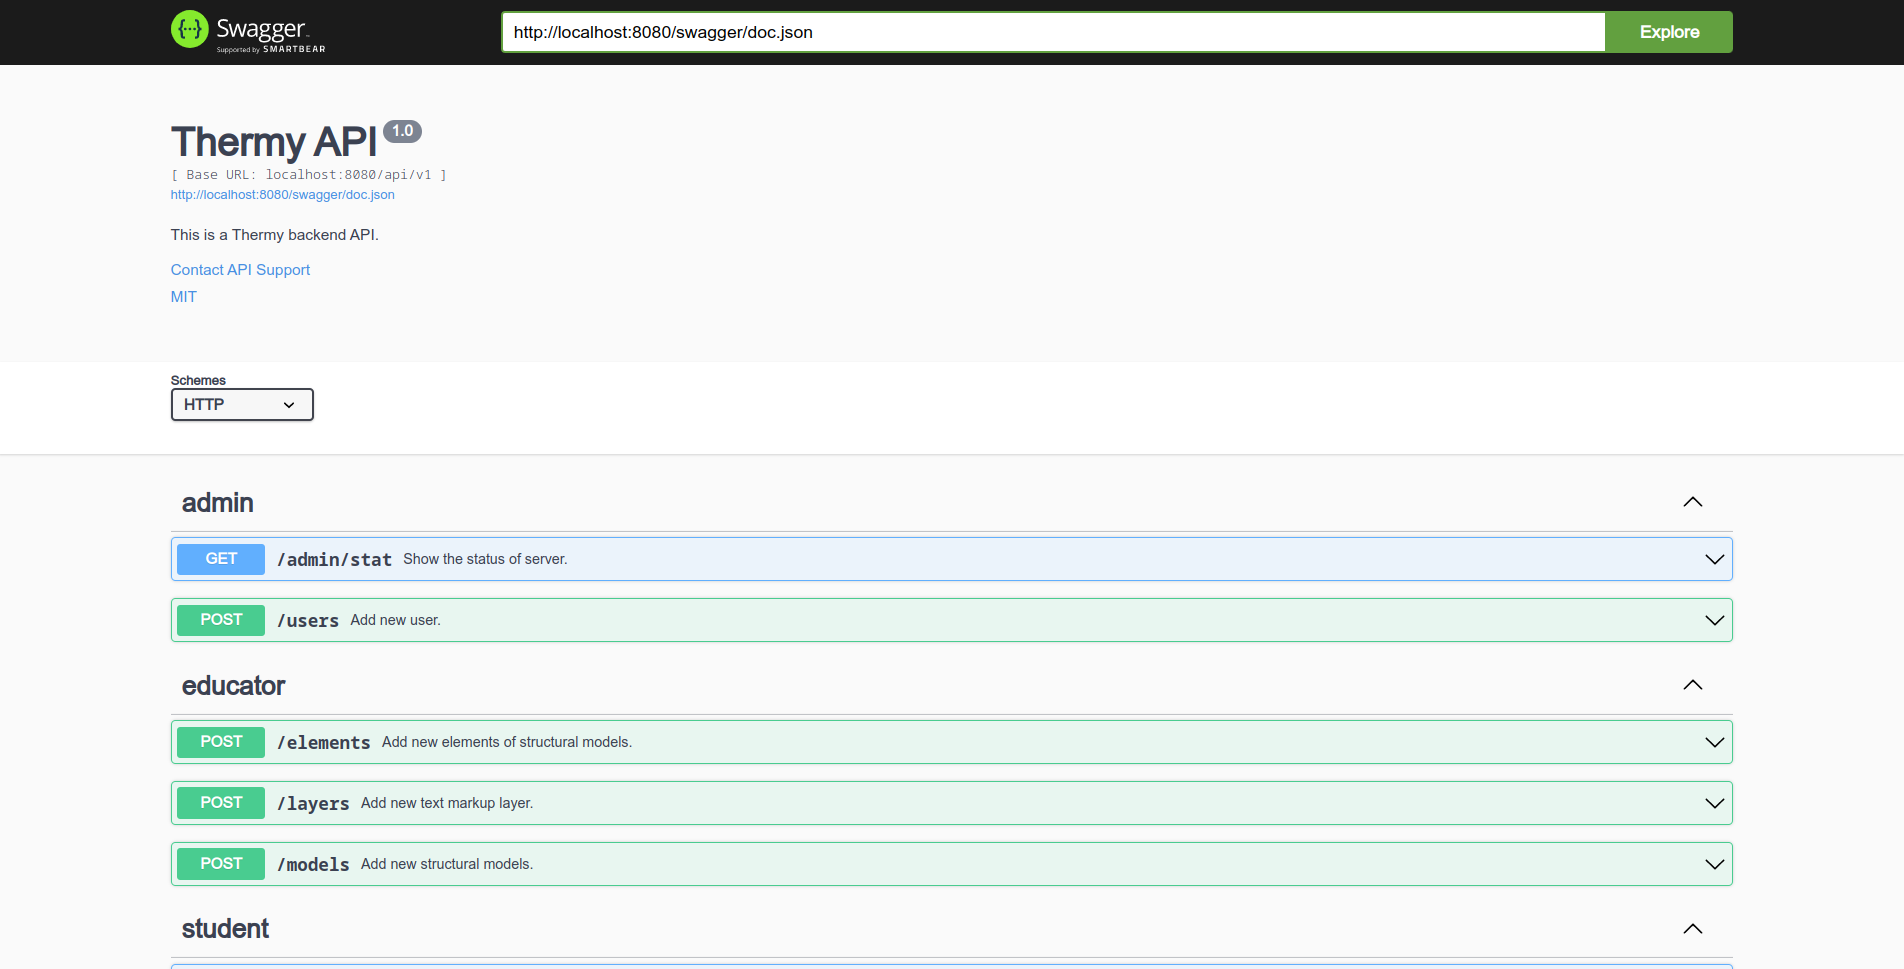
\includegraphics[width=\textwidth ]{img/Swagger/main.png}
	\caption{Главная страница Swagger UI}
	\label{fig:swagger_main}
\end{figure} 
	
\begin{figure}[h]
	\centering
	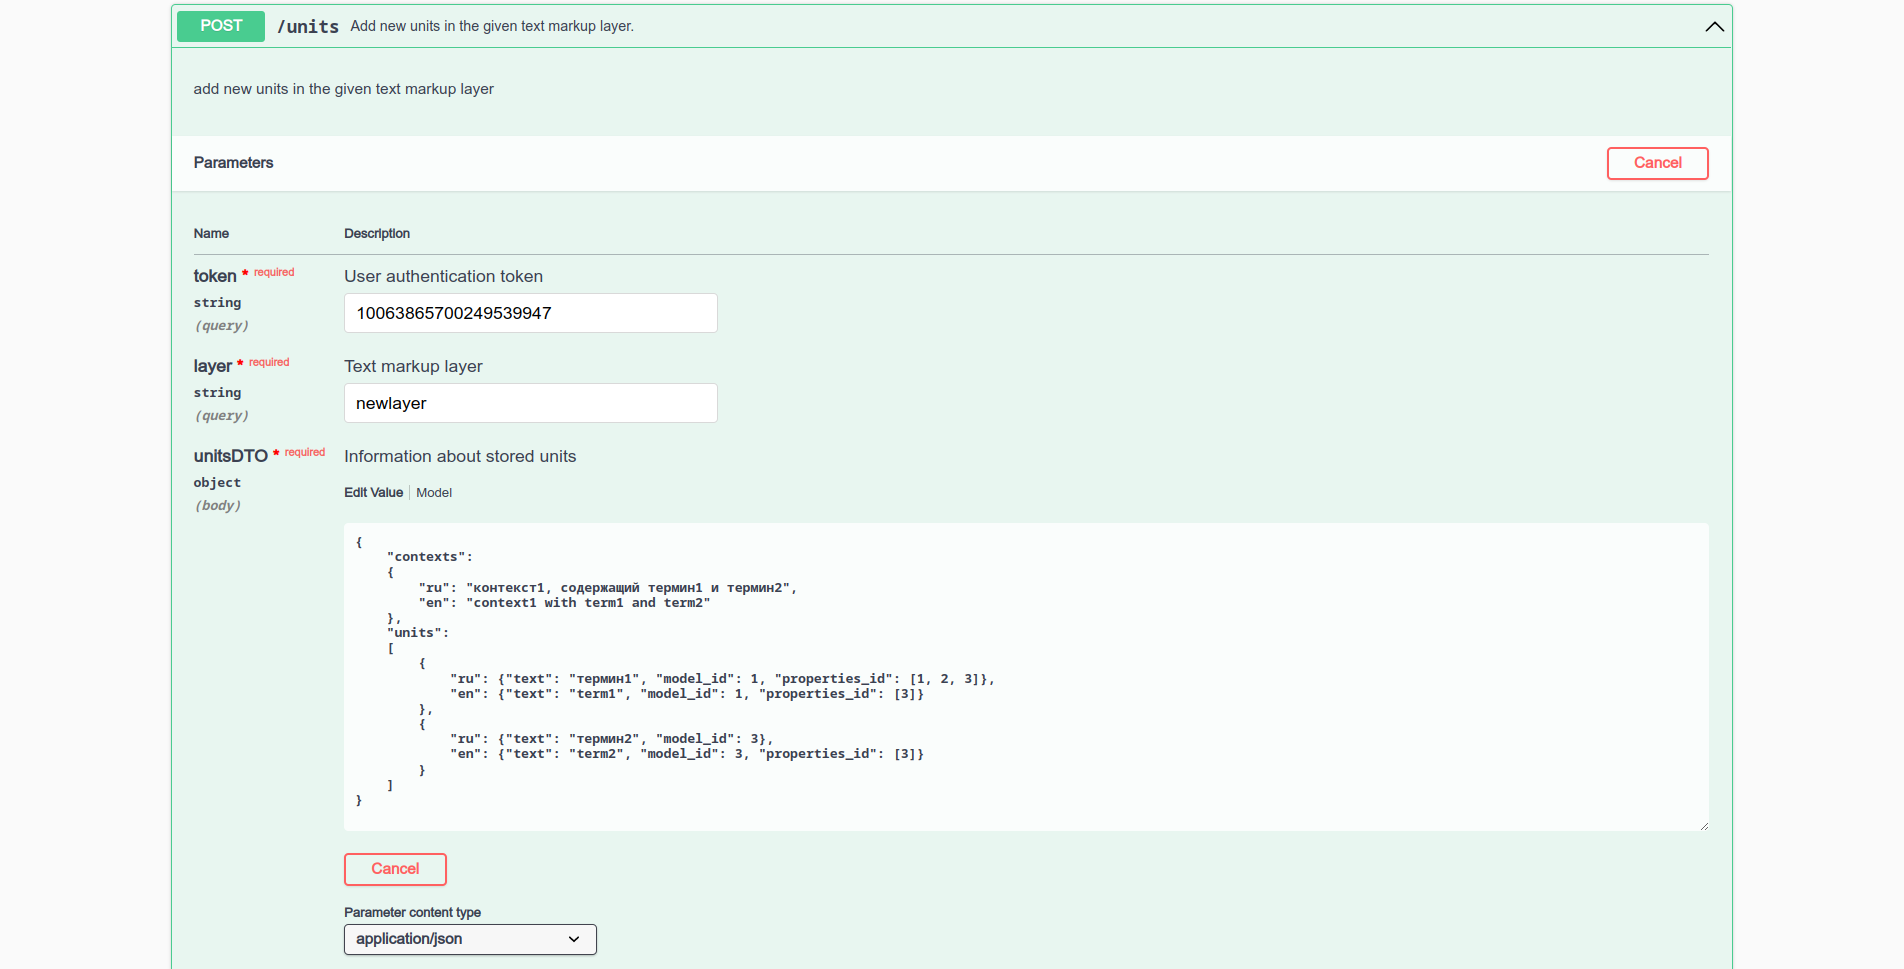
\includegraphics[width=\textwidth ]{img/Swagger/form_request.png}
	\caption{Пример заполнения формы для сохранения терминов с помощью Swagger UI}
	\label{fig:swagger_form_request}
	
	\centering
	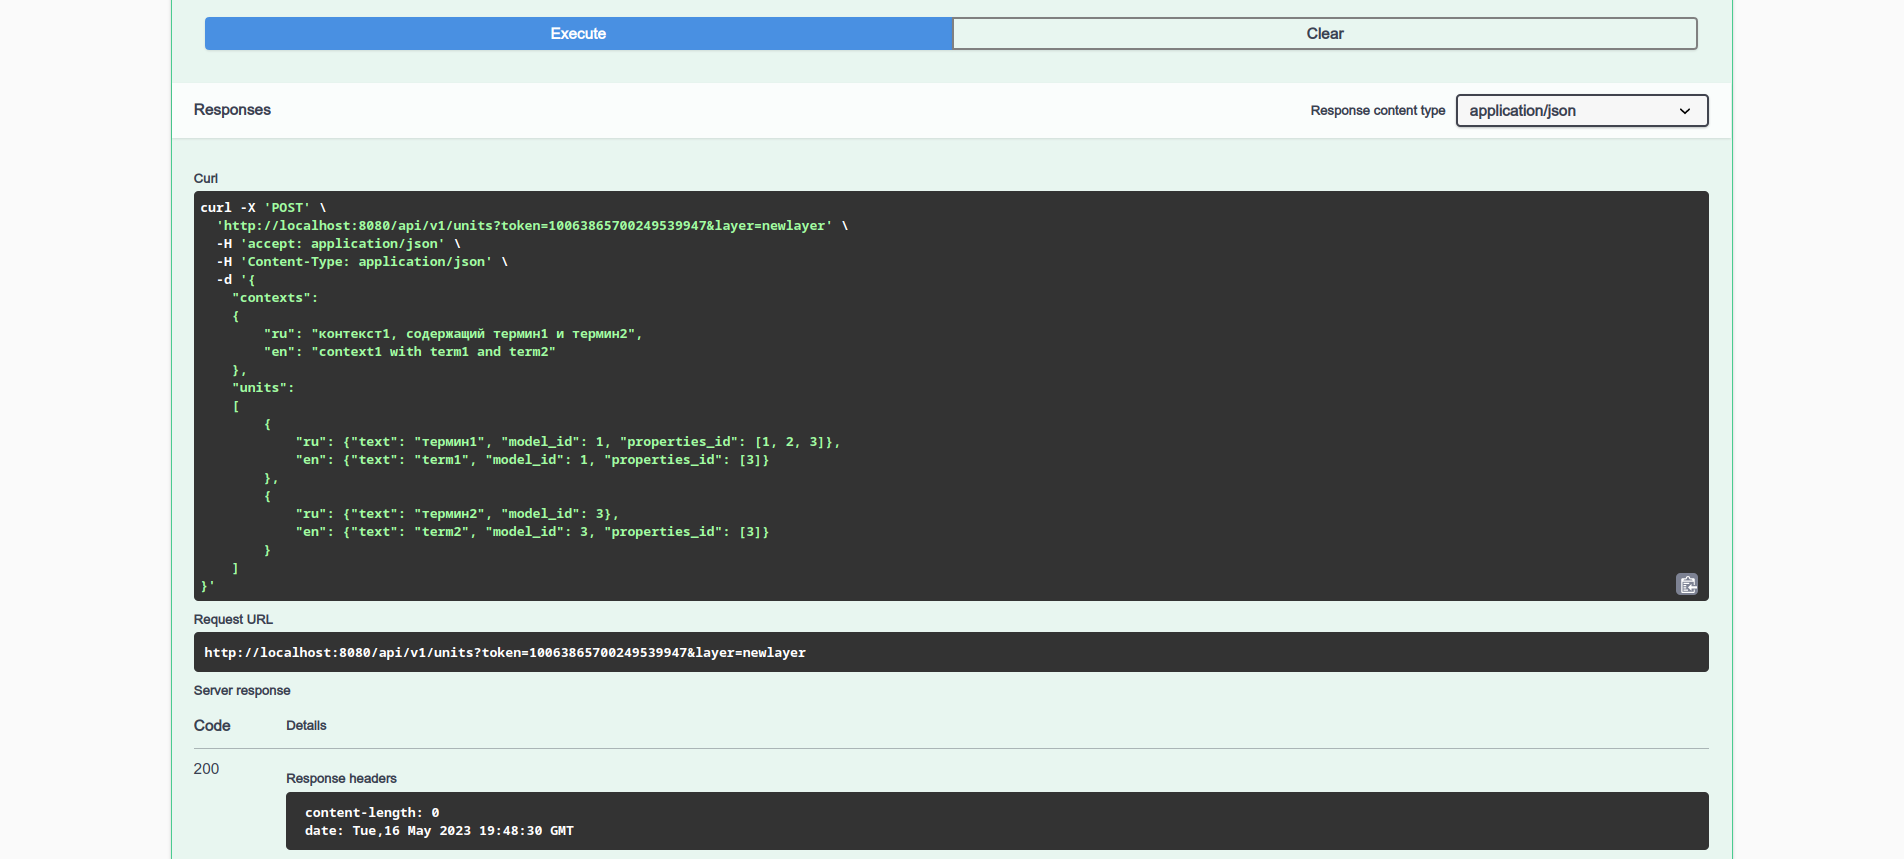
\includegraphics[width=\textwidth ]{img/Swagger/form_response.png}
	\caption{Пример ответа на запрос сохранения терминов с помощью Swagger UI}
	\label{fig:swagger_form_response}
\end{figure} 

\clearpage



\subsection*{Вывод из технологической части}

В данном разделе были приведены детали реализации ПО, использующего следующие технологии.

\begin{enumerate}[label*=\arabic*.]
	\item Golang --- язык для написания серверной части приложения.
	\item PostgreSQL --- основное хранилище данных.
	\item PgAdmin --- инструмент для администрирования PostgreSQL.
	\item PL/pgSQL --- расширение языка SQL, использовавшееся для написания хранимых процедур базы данных.
	\item Redis --- кеш данных пользовательских сессий.
	\item InfluxDB --- сервер логов.
	\item Swagger --- инструмент документирования API сервера.
	\item Docker --- платформа для для автоматизации развёртывания и управления приложениями.
	\item Docker Compose --- оркестратор контейнеров.
\end{enumerate}

\pagebreak